\documentclass{ctexart}
\usepackage[utf8]{inputenc}
\usepackage{geometry}
\usepackage{graphicx}
\usepackage{amsmath}
\usepackage{amssymb}
\usepackage{enumitem}
\usepackage{xcolor}
\usepackage{listings}
\usepackage{threeparttable}
\usepackage{multirow}
\usepackage{longtable}
\geometry{a4paper,left=2cm,right=2cm,top=1.5cm,bottom=1cm}
\newfontfamily\courier{Consolas}
\lstset{linewidth=1.1\textwidth,
		numbers=left, %设置行号位置 
		basicstyle=\small\courier,
		numberstyle=\tiny\courier, %设置行号大小  
		keywordstyle=\color{blue}\courier, %设置关键字颜色  
		%identifierstyle=\bf,
		commentstyle=\it\color[cmyk]{1,0,1,0}\courier, %设置注释颜色 
		stringstyle=\it\color[RGB]{128,0,0}\courier,
		%framexleftmargin=10mm,
		frame=single, %设置边框格式  
		backgroundcolor=\color[RGB]{245,245,244},
		%escapeinside=``, %逃逸字符(1左面的键),用于显示中文  
		breaklines, %自动折行  
		extendedchars=false, %解决代码跨页时,章节标题,页眉等汉字不显示的问题  
		xleftmargin=2em,xrightmargin=2em, aboveskip=1em, %设置边距  
		tabsize=4, %设置tab空格数  
		showspaces=false %不显示空格  
		basicstyle=\small\courier
	   }
\newcommand{\subsubsubsection}[1]{\paragraph{#1}\mbox{}\\}
\setcounter{secnumdepth}{4} % how many sectioning levels to assign numbers to
\setcounter{tocdepth}{4} % how many sectioning levels to show in ToC
\title{微分方程数值解 - 第十二章上机作业}
\author{樊睿 强基数学 2001 班}
\date{2023年6月16日}

\begin{document}

\maketitle

\begin{abstract}
	本项目实现了三种解热方程的MOL方法和五种解对流方程的MOL方法,并通过作出它们对给定齐次初边值问题的解在不同时间的图像分析它们的收敛性和稳定性。
\end{abstract}

\section{类的设计}
所有MOL方法均从基类MOL继承。

所有MOL方法都用单步法作为解初值问题的方法,因此Solve函数可以统一实现。

另外定义init函数求出$k,h,r,\mu$以及初值。

\begin{lstlisting}[language=c++]
class MOL {
protected:
	string name;
	int n, m;
	double k, h;
	vector<Colvec<double>> u;
	virtual void init(const Function_2D<double>& f, const double& nu, const double& T, const int& n, const int& m) = 0;
	virtual void step(const Function_2D<double>& f, const int& n) = 0;
public:
	virtual vector<Colvec<double>> Solve(const Function_2D<double>& f, const double& nu, const double& T, const int& n, const int& m) {
		init(f, nu, T, n, m);
		for (int i = 1; i <= n; ++ i) step(f, i-1);
		return u;
	}
};

class MOL_for_heat : public MOL {
protected:
	double r;
	virtual void init(const Function_2D<double>& f, const double& nu, const double& T, const int& n, const int& m) {
		this->n = n, this->m = m;
		k = T/n, h = 1.0/m, r = nu * k / (h*h);
		u.resize(n+1);
		for (int i = 0; i <= n; ++ i) u[i] = Colvec<double>(m+1);
		for (int i = 0; i <= m; ++ i) u[0][i] = f(0, i*h);
	}
};

class MOL_adv : public MOL {
protected:
	double mu;
	virtual void init(const Function_2D<double>& f, const double& nu, const double& T, const int& n, const int& m) {
		this->n = n, this->m = m;
		k = T/n, h = 1.0/m, mu = nu * k / (h*h);
		u.resize(n+1);
		for (int i = 0; i <= n; ++ i) u[i] = Colvec<double>(m+1);
		for (int i = 0; i <= m; ++ i) u[0][i] = f(0, i*h);
	}
};
\end{lstlisting}

\section{热方程初边值问题的MOL方法}

热方程是形如 $u_t=\nu u_{xx}$ 的偏微分方程。

热方程的初边值问题就是给出 $u(0,x)=f(x)$ 和 $u(t,0)=g_0(t),u(t,1)=g_1(t)$。

齐次初边值问题就是 $g_0=g_1=0$。

对于初边值问题,我们的解法一般是先利用第7章的空间离散方法得到常微分方程组,再利用第11章的数值方法求解。

本节中取 $a=1,f(x) = \max(0,1+20|x-\dfrac 12|)$。我们可以用傅里叶变换计算出它的级数形式精确解。取前 $100$ 项之和作为其真解。

固定网格大小 $h=0.05$。

\subsection{$theta$-Methods}

$theta$-Methods是一类一阶时间离散、二阶空间离散的数值方法。它的基本思路是:空间导数使用第七章的二阶有限差分法离散,时间导数使用向前Euler格式和向后Euler格式的加权平均。

它使用的时间离散公式为

\begin{equation}
	U^{n+1} = \theta f(U^{n+1}) + (1-\theta) f(U^n).
\end{equation}

将其与空间离散

\begin{equation}
	U'=Au
\end{equation}

相结合,可得最终方程

\begin{equation}
	-r\theta U_{i-1}^{n+1} + (1+2r\theta) U_i^{n+1} - r\theta U_{i+1}^{n+1} = (1-\theta) U_{i-1}^n + (1+2(1-\theta)) U_i^n + (1-\theta) U_{i+1}^n.
\end{equation}

这样每一步需要解一个线性方程组。使用带稀疏优化的高斯消元法(见第七章报告)解,当时间步数为$n$、空间步数为$m$时,复杂度为$O(nm^2)$。

所有$\theta$-Methods都是一阶时间、二阶空间收敛的。但$\theta$和$r$的关系的会导致稳定性的差异。

\subsubsection{FTCS方法}

FTCS方法是$\theta=0$的$\theta$方法,即完全使用向前Euler法做时间离散。它是无条件不稳定的。

图\ref{ftcs1}至图\ref{ftcs6}分别是FTCS方法在$r=\dfrac 12$和$r=1$时,$t=k,2k,10k$时的图像。蓝色实线为真解。

\begin{figure}[htbp]
	\begin{minipage}{5cm}
		\centering
		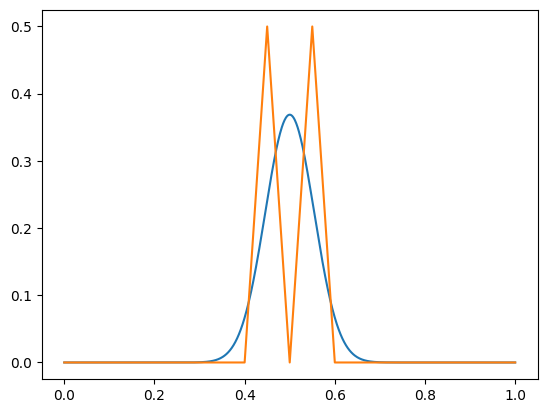
\includegraphics[width = 3cm, height = 3cm]{2-3-1.png}
		\caption{FTCS, $r=\frac 12,N=1$}
		\label{ftcs1}
	\end{minipage}
	\begin{minipage}{5cm}
		\centering
		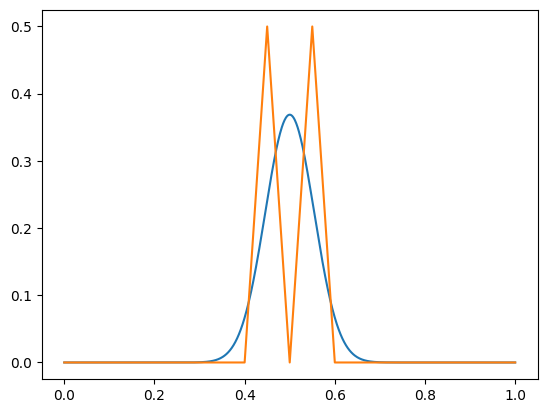
\includegraphics[width = 3cm, height = 3cm]{2-3-2.png}
		\caption{FTCS, $r=\frac 12,N=2$}
		\label{ftcs2}
	\end{minipage}
	\begin{minipage}{5cm}
		\centering
		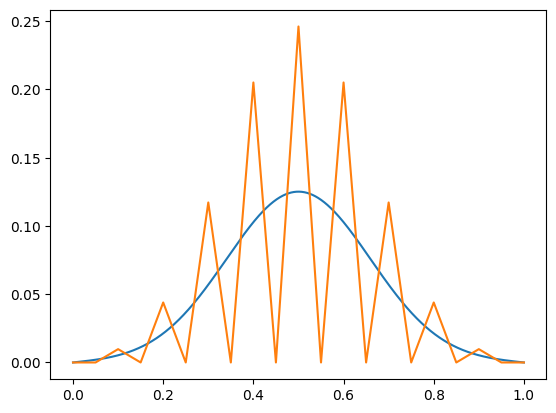
\includegraphics[width = 3cm, height = 3cm]{2-3-3.png}
		\caption{FTCS, $r=\frac 12,N=10$}
		\label{ftcs3}
	\end{minipage}
	\begin{minipage}{5cm}
		\centering
		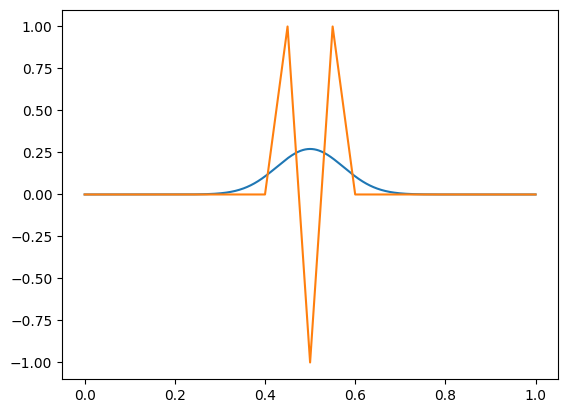
\includegraphics[width = 3cm, height = 3cm]{2-4-1.png}
		\caption{FTCS, $r=1,N=1$}
		\label{ftcs4}
	\end{minipage}
	\begin{minipage}{5cm}
		\centering
		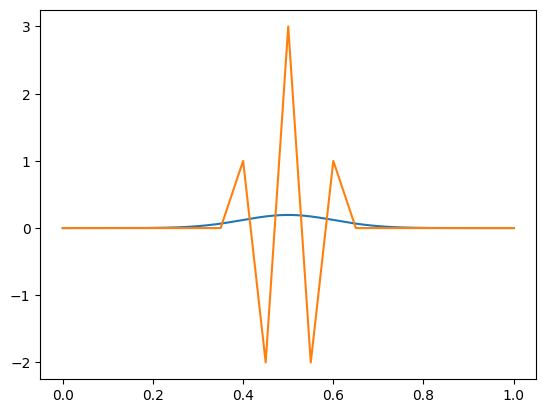
\includegraphics[width = 3cm, height = 3cm]{2-4-2.png}
		\caption{FTCS, $r=1,N=2$}
		\label{ftcs5}
	\end{minipage}
	\begin{minipage}{5cm}
		\centering
		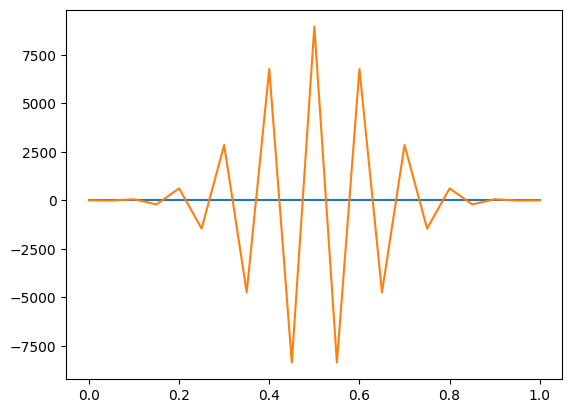
\includegraphics[width = 3cm, height = 3cm]{2-4-3.png}
		\caption{FTCS, $r=1,N=10$}
		\label{ftcs6}
	\end{minipage}
\end{figure}

可见FTCS方法对于这样一个简单的能写出解析解的方程都是不稳定的。因此这样一个方法没有任何实用价值,我们也没有必要进一步分析它的收敛阶了。

\subsubsection{Crank-Nicolson方法}

Crank-Nicolson方法是$\theta=\dfrac 12$的$\theta$-Method。

图\ref{CN1}至图\ref{CN6}分别是Crank-Nicolson方法在$r=1$和$r=\dfrac 1{2h}$时,$t=k,2k,10k$时的图像。蓝色实线为真解。

\begin{figure}[htbp]
	\begin{minipage}{5cm}
		\centering
		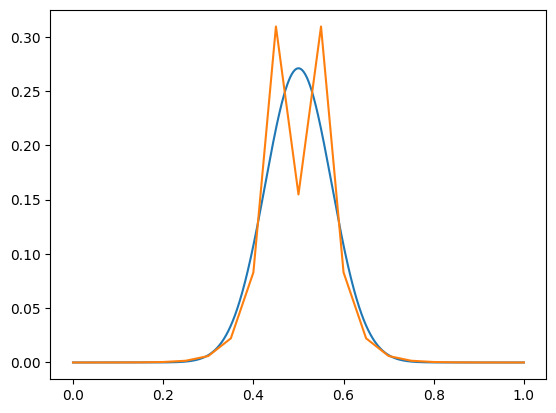
\includegraphics[width = 3cm, height = 3cm]{1-1-1.png}
		\caption{C-N, $r=1,N=1$}
		\label{CN1}
	\end{minipage}
	\begin{minipage}{5cm}
		\centering
		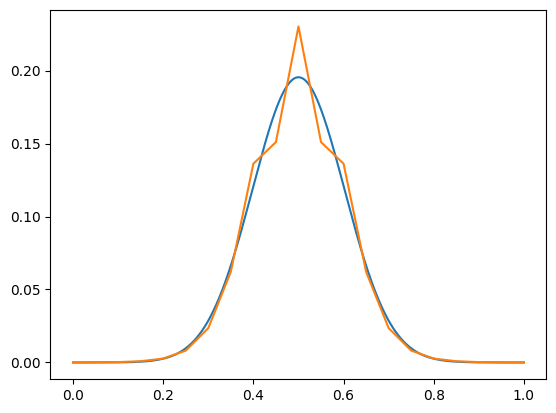
\includegraphics[width = 3cm, height = 3cm]{1-1-2.png}
		\caption{C-N, $r=1,N=2$}
		\label{CN2}
	\end{minipage}
	\begin{minipage}{5cm}
		\centering
		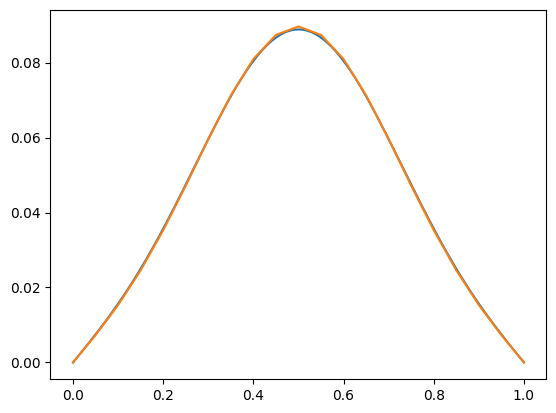
\includegraphics[width = 3cm, height = 3cm]{1-1-3.png}
		\caption{C-N, $r=1,N=10$}
		\label{CN3}
	\end{minipage}
	\begin{minipage}{5cm}
		\centering
		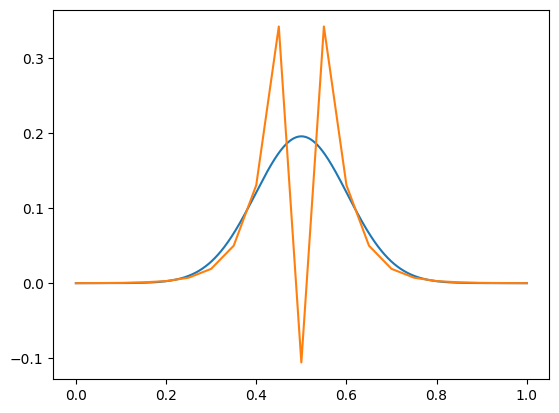
\includegraphics[width = 3cm, height = 3cm]{1-2-1.png}
		\caption{C-N, $r=\frac 1{2h},N=1$}
		\label{CN4}
	\end{minipage}
	\begin{minipage}{5cm}
		\centering
		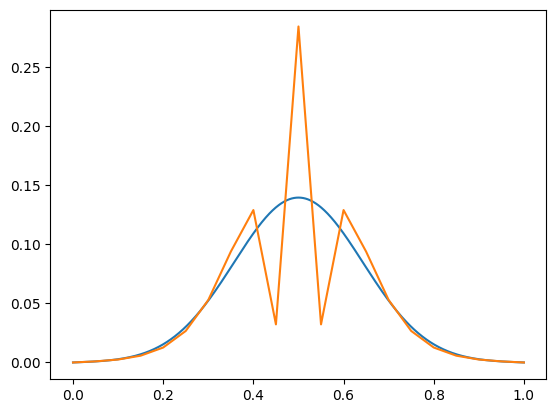
\includegraphics[width = 3cm, height = 3cm]{1-2-2.png}
		\caption{C-N, $r=\frac 1{2h},N=2$}
		\label{CN5}
	\end{minipage}
	\begin{minipage}{5cm}
		\centering
		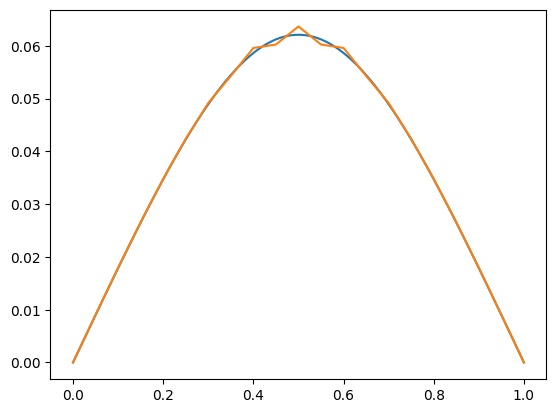
\includegraphics[width = 3cm, height = 3cm]{1-2-3.png}
		\caption{C-N, $r=\frac 1{2h},N=10$}
		\label{CN6}
	\end{minipage}
\end{figure}

可见$r=1$时方法的收敛速度更快。这也体现了方法的空间收敛阶是时间收敛阶的2倍。

下面对它的收敛阶进行详细分析。我们先固定空间步长改变时间步长,再固定时间步长改变空间步长,并限定终结时间为 $T=1$:

\begin{table}\centering
	\begin{tabular}{|c|c|c|c|c|}
	\hline
	时间步数 & 网格数量 & 误差 & 时间 & 收敛阶\\ \cline{1-5}
	128 & 128 & 1.91e-03 & 68  & - \\ \cline{1-5}
	256 & 128 & 6.01e-05 & 116 & 4.99 \\ \cline{1-5}
	512 & 128 & 2.21e-08 & 238 & 11.44\\ \cline{1-5}
	16384 & 8 & 7.19e-06 & 92 & - \\ \cline{1-5}
	16384 & 16 & 1.10e-06 & 212 & 2.71 \\ \cline{1-5}
	16384 & 32 & 3.80e-07 & 608 & 1.53 \\ \cline{1-5}
	\end{tabular}
	\caption{Crank-Nicolson方法的误差和收敛阶}
\end{table}

虽然Crank-Nicolson方法的收敛阶理论上是$O(k^2+h^2)$,但实际上极其不稳定。

这可能是$k$和$h$的交叉影响造成的。另外,Crank-Nicolson方法所用的时间离散格式为显式中点法,它不是刚性稳定的,因此会造成收敛阶的混乱。

\subsubsection{BTCS方法}

BTCS方法是$\theta=1$的$\theta$-Method。即完全用向后Euler格式做时间离散。

图\ref{btcs1}至图\ref{btcs6}分别是Crank-Nicolson方法在$r=1$和$r=2$时,$t=k,2k,10k$时的图像。蓝色实线为真解。

\begin{figure}[htbp]
	\begin{minipage}{5cm}
		\centering
		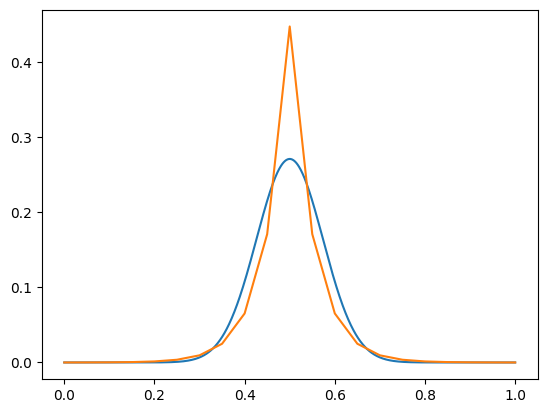
\includegraphics[width = 3cm, height = 3cm]{1-3-1.png}
		\caption{BTCS, $r=1,N=1$}
		\label{btcs1}
	\end{minipage}
	\begin{minipage}{5cm}
		\centering
		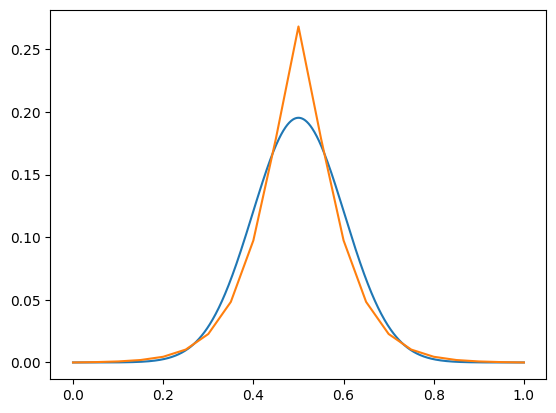
\includegraphics[width = 3cm, height = 3cm]{1-3-2.png}
		\caption{BTCS, $r=1,N=2$}
		\label{btcs2}
	\end{minipage}
	\begin{minipage}{5cm}
		\centering
		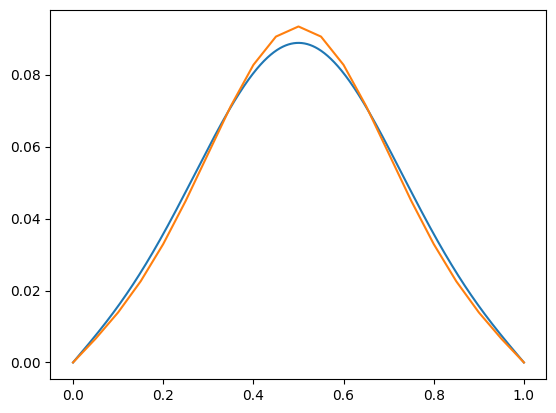
\includegraphics[width = 3cm, height = 3cm]{1-3-3.png}
		\caption{BTCS, $r=1,N=10$}
		\label{btcs3}
	\end{minipage}
	\begin{minipage}{5cm}
		\centering
		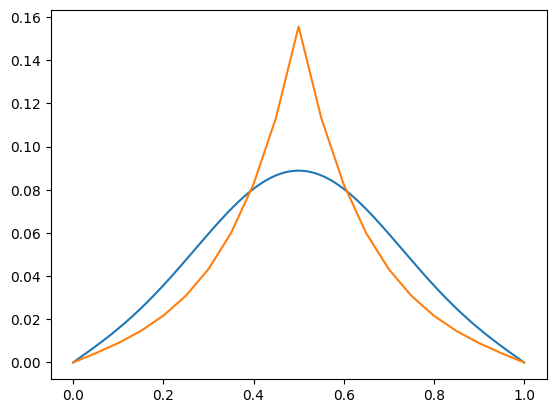
\includegraphics[width = 3cm, height = 3cm]{2-1-1.png}
		\caption{BTCS, $r=2,N=1$}
		\label{btcs4}
	\end{minipage}
	\begin{minipage}{5cm}
		\centering
		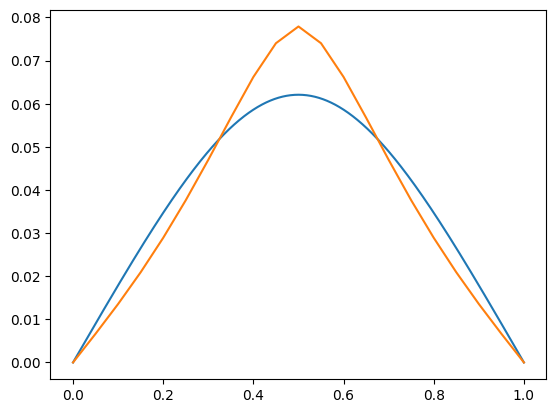
\includegraphics[width = 3cm, height = 3cm]{2-1-2.png}
		\caption{BTCS, $r=2,N=2$}
		\label{btcs5}
	\end{minipage}
	\begin{minipage}{5cm}
		\centering
		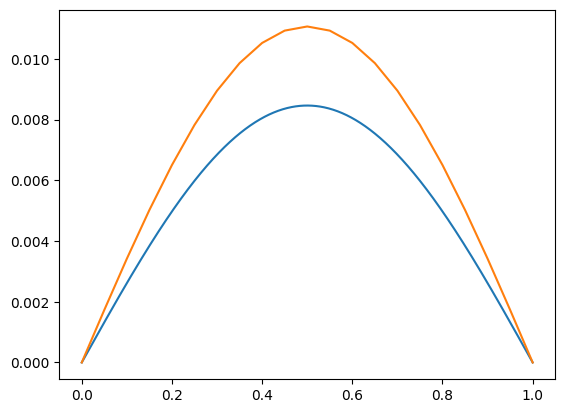
\includegraphics[width = 3cm, height = 3cm]{2-1-3.png}
		\caption{BTCS, $r=2,N=10$}
		\label{btcs6}
	\end{minipage}
\end{figure}

可见 $r=1$ 时方法的收敛速度更快。这也体现了方法的空间收敛阶是时间收敛阶的2倍。

下面对它的收敛阶进行详细分析。我们先固定空间步长改变时间步长,再固定时间步长改变空间步长,并限定终结时间为 $T=1$:

\begin{table}\centering
	\begin{tabular}{|c|c|c|c|c|}
	\hline
	时间步数 & 网格数量 & 误差 & 时间 & 收敛阶\\ \cline{1-5}
	128 & 128 & 1.63e-06 & 79  & - \\ \cline{1-5}
	256 & 128 & 7.75e-07 & 107 & 1.07 \\ \cline{1-5}
	512 & 128 & 3.86e-07 & 228 & 1.00\\ \cline{1-5}
	16384 & 8 & 7.22e-06 & 94 & - \\ \cline{1-5}
	16384 & 16 & 1.12e-06 & 194 & 2.69 \\ \cline{1-5}
	16384 & 32 & 3.92e-07 & 528 & 1.51 \\ \cline{1-5}
	\end{tabular}
	\caption{BTCS方法的误差和收敛阶}
\end{table}

BTCS方法的收敛阶理论上是$O(k+h^2)$,但实际上和理论也有较大差别,特别是空间离散。

这可能是因为空间离散需要解多个条件数很大的方程组,而且随着$m$的增大,方程组的条件数是平方级增大的。这也就导致了收敛阶随$m$的增大而减小。

\subsection{RK方法与二阶空间离散结合}

Euler方法在时间上是一阶的,阶数太低了。我们需要一个高阶的单步方法。因此考虑11.6节的RK方法。

我们直接对一般的RK方法结合二阶空间离散导出MOL。

用空间二阶离散,得到半离散格式:

\begin{equation}
	U' = \dfrac {U_{i-1} - 2U_i + U_{i+1}}{h^2}.
\end{equation}

其中 $U=\{U_i\}_{i=0}^m$ 是 $m+1$ 维空间离散的向量。

根据RK方法

\begin{equation}	
\begin{aligned}
	y^j = f(U^n + k\sum_{l=1}^s a_{j,l}y^l),\\
	U^{n+1} = U^n + \sum_{j=1}^s b_jy^j.
\end{aligned}
\end{equation}

我们有

\begin{equation}
\begin{aligned}
	y_i^j = \dfrac 1{h^2}(U^n_{i-1} - 2U^n_i + U^n_{i+1} + k\sum_{l=1}^s (y^l_{i-1} - 2y^l_i + y^l_{i+1})).\\
	U^{n+1} = U^n + \sum_{j=1}^s b_jy^j.
\end{aligned}
\end{equation}

这样我们只需求解一个 $s(m+1)$ 维线性方程组即可。

\begin{lstlisting}
class MOL_heat_with_RK : public MOL_for_heat {
	protected:
		int s;
		vector<vector<double>> a;
		vector<double> b;
		int id(int i, int j) {
			return j*(m+1)+i;
		}
		virtual void step(const Function_2D<double>& f, const int& n) {
			Matrix<double> coef(s*(m+1), s*(m+1));
			Colvec<double> rhs(s*(m+1));
			for (int i = 1; i < m; ++ i) {
				for (int j = 0; j < s; ++ j) {
					for (int l = 0; l < s; ++ l) {
						coef[id(i,j)][id(i,l)] += 2*r*a[j][l];
						coef[id(i,j)][id(i-1,l)] -= r*a[j][l];
						coef[id(i,j)][id(i+1,l)] -= r*a[j][l];
					}
					coef[id(i,j)][id(i,j)] += 1;
					rhs[id(i,j)] = r * (u[n][i-1] - 2*u[n][i] + u[n][i+1]) / k;
				}
			}
			for (int j = 0; j < s; ++ j) {
				coef[id(0,j)][id(0,j)] = 1, rhs[id(0,j)] = 0;
				coef[id(m,j)][id(m,j)] = 1, rhs[id(m,j)] = 0;
			}
			Colvec<double> ys = Gauss_Improved_Solve(coef, rhs);
			vector<Colvec<double>> y(s);
			for (int j = 0; j < s; ++ j) y[j] = split(ys, j*(m+1), (j+1)*(m+1));
			u[n+1] = u[n];
			for (int j = 0; j < s; ++ j) u[n+1] += k * b[j] * y[j];
		}
	};
\end{lstlisting}

\subsubsection{Collocation-Method}

考虑例 11.258 的 Collocation-Method。

图\ref{CM1}至图\ref{CM6}分别是Crank-Nicolson方法在$r=1$和$r=\dfrac 1{2h}$时,$t=k,2k,10k$时的图像。蓝色实线为真解。

\begin{figure}[htbp]
	\begin{minipage}{5cm}
		\centering
		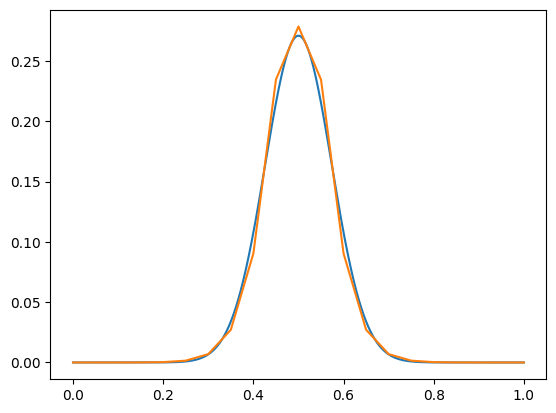
\includegraphics[width = 3cm, height = 3cm]{1-4-1.png}
		\caption{C-M, $r=1,N=1$}
		\label{CM1}
	\end{minipage}
	\begin{minipage}{5cm}
		\centering
		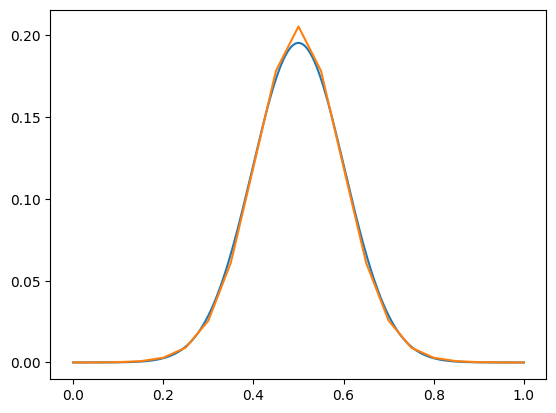
\includegraphics[width = 3cm, height = 3cm]{1-4-2.png}
		\caption{C-M, $r=1,N=2$}
		\label{CM2}
	\end{minipage}
	\begin{minipage}{5cm}
		\centering
		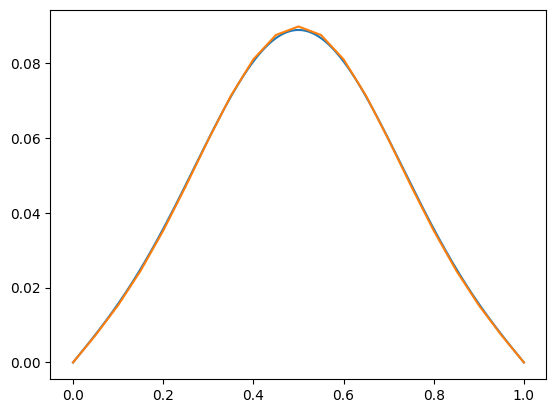
\includegraphics[width = 3cm, height = 3cm]{1-4-3.png}
		\caption{C-M, $r=1,N=10$}
		\label{CM3}
	\end{minipage}
	\begin{minipage}{5cm}
		\centering
		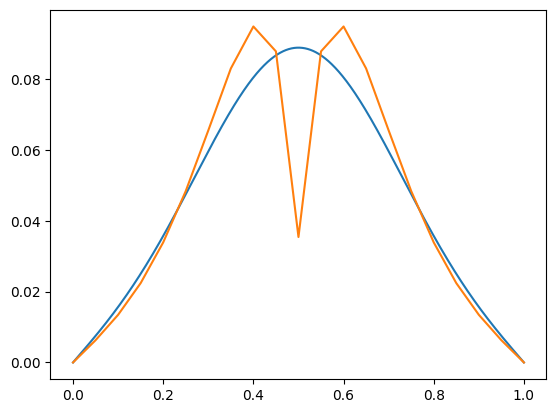
\includegraphics[width = 3cm, height = 3cm]{2-2-1.png}
		\caption{C-M, $r=\frac 1{2h},N=1$}
		\label{CM4}
	\end{minipage}
	\begin{minipage}{5cm}
		\centering
		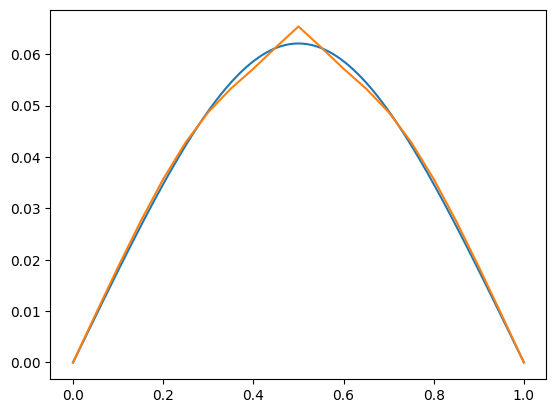
\includegraphics[width = 3cm, height = 3cm]{2-2-2.png}
		\caption{C-M, $r=\frac 1{2h},N=2$}
		\label{CM5}
	\end{minipage}
	\begin{minipage}{5cm}
		\centering
		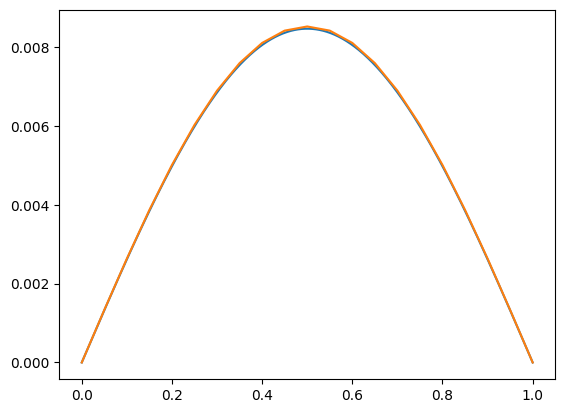
\includegraphics[width = 3cm, height = 3cm]{2-2-3.png}
		\caption{C-M, $r=\frac 1{2h},N=10$}
		\label{CM6}
	\end{minipage}
\end{figure}

可见$r=1$时方法的收敛速度更快。但$r=\dfrac 1{2h}$时同样很快收敛。

下面对它的收敛阶进行详细分析。我们先固定空间步长改变时间步长,再固定时间步长改变空间步长,并限定终结时间为 $T=1$:

\begin{table}\centering
	\begin{tabular}{|c|c|c|c|c|}
	\hline
	时间步数 & 网格数量 & 误差 & 时间 & 收敛阶\\ \cline{1-5}
	2 & 128 & 4.34e-04 & 22  & - \\ \cline{1-5}
	4 & 128 & 3.51e-06 & 43 & 6.95 \\ \cline{1-5}
	8 & 128 & 6.82e-07 & 85 & 2.36\\ \cline{1-5}
	128 & 8 & 7.19e-06 & 3 & - \\ \cline{1-5}
	128 & 16 & 1.10e-06 & 12 & 2.71 \\ \cline{1-5}
	128 & 32 & 3.80e-07 & 59 & 1.53 \\ \cline{1-5}
	\end{tabular}
	\caption{Collocation方法的误差和收敛阶}
\end{table}

Collocation方法的理论收敛阶是 $O(k^3+h^2)$,但事实上,因为时间上收敛阶太高,$n$取$8$时已经几乎达到了空间的上限。因此难以分析其真实的时间收敛阶。

\subsubsection{Collocation-Method}

考虑例11.227的一阶Gauss-Legrend方法。

图\ref{GL1}至图\ref{GL6}分别是Gauss-Legrend方法在$r=1$和$r=\dfrac 1{2h}$时,$t=k,2k,10k$时的图像。蓝色实线为真解。

\begin{figure}[htbp]
	\begin{minipage}{5cm}
		\centering
		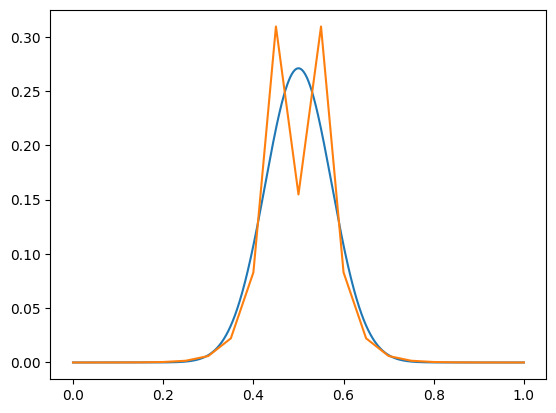
\includegraphics[width = 3cm, height = 3cm]{2-5-1.png}
		\caption{GL, $r=1,N=1$}
		\label{GL1}
	\end{minipage}
	\begin{minipage}{5cm}
		\centering
		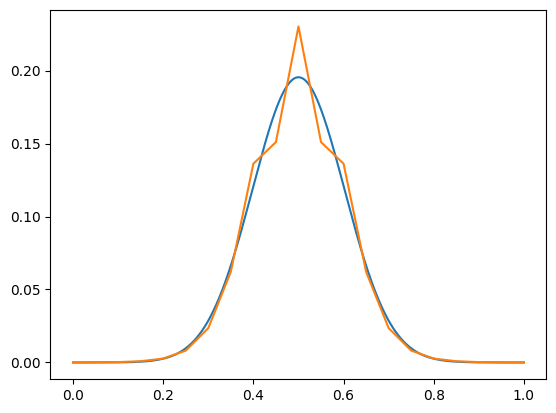
\includegraphics[width = 3cm, height = 3cm]{2-5-2.png}
		\caption{GL, $r=1,N=2$}
		\label{GL2}
	\end{minipage}
	\begin{minipage}{5cm}
		\centering
		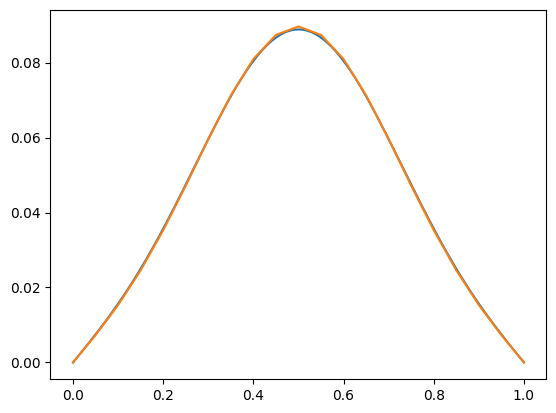
\includegraphics[width = 3cm, height = 3cm]{2-5-3.png}
		\caption{GL, $r=1,N=10$}
		\label{GL3}
	\end{minipage}
	\begin{minipage}{5cm}
		\centering
		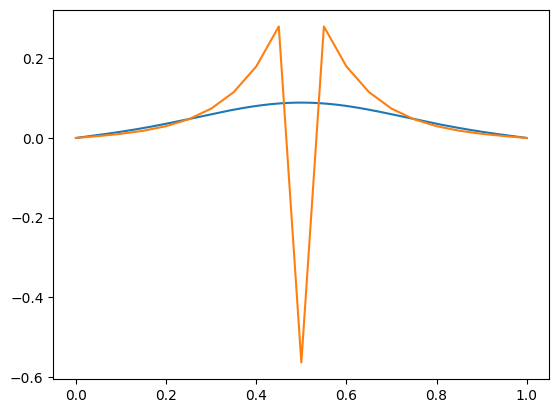
\includegraphics[width = 3cm, height = 3cm]{2-6-1.png}
		\caption{GL, $r=\frac 1{2h},N=1$}
		\label{GL4}
	\end{minipage}
	\begin{minipage}{5cm}
		\centering
		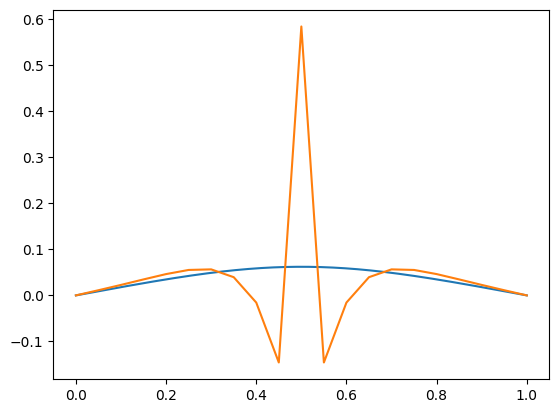
\includegraphics[width = 3cm, height = 3cm]{2-6-2.png}
		\caption{GL, $r=\frac 1{2h},N=2$}
		\label{GL5}
	\end{minipage}
	\begin{minipage}{5cm}
		\centering
		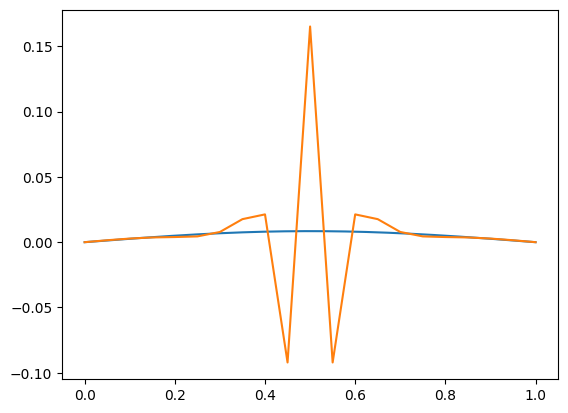
\includegraphics[width = 3cm, height = 3cm]{2-6-3.png}
		\caption{GL, $r=\frac 1{2h},N=10$}
		\label{GL6}
	\end{minipage}
\end{figure}

下面对它的收敛阶进行详细分析。我们先固定空间步长改变时间步长,再固定时间步长改变空间步长,并限定终结时间为 $T=1$:

\begin{table}\centering
	\begin{tabular}{|c|c|c|c|c|}
	\hline
	时间步数 & 网格数量 & 误差 & 时间 & 收敛阶\\ \cline{1-5}
	128 & 128 & 1.91e-03 & 53  & - \\ \cline{1-5}
	256 & 128 & 6.01e-05 & 100 & 6.95 \\ \cline{1-5}
	512 & 128 & 2.21e-08 & 219 & 2.36\\ \cline{1-5}
	16384 & 8 & 7.19e-06 & 133 & - \\ \cline{1-5}
	16384 & 16 & 1.10e-06 & 237 & 2.71 \\ \cline{1-5}
	16384 & 32 & 3.80e-07 & 564 & 1.53 \\ \cline{1-5}
	\end{tabular}
	\caption{一阶Gauss-Legrend方法的误差和收敛阶}
\end{table}

观察图\ref{CN1}到图\ref{CN3}和图\ref{GL1}到图\ref{GL3},我们不难发现,这几张图一模一样!再观察两张表,所有数据也都是一样的。

这是因为这两种方法的时间离散本质上是相同的。因此两种MOL也是本质相同的。

\section{对流方程周期解的MOL方法}

对流方程是形如 $u_t+au_x=0$ 的偏微分方程。

对流方程的初值问题即给出 $u(0,x)=f(x)$。

由于研究的是周期解,所以无需给出边值条件。

本节中取 $a=1,f(x) = \exp\{-20(x-2)^2\} + \exp\{-(x-5)^2\}$。

其真解为 $u(t,x) = \exp\{-20(x-t-2)^2\} + \exp\{-(x-t-5)^2\}$。

网格大小 $h$ 取 $0.05$,终止时间 $T$ 取 $17$,循环长度取 $25$。

\subsection{LeapFrog方法}

LeapFrog方法采用最朴素的离散格式,在时间和空间上均采用一阶离散。即

\begin{equation}
	\dfrac {U^{n+1}_i-U^{n-1}_i}{2k} = -a\dfrac {U^n_{i+1} - U^n_{i-1}}{2h}.
\end{equation}

这个方法需要用到 $U^{n-1}$。当 $n=0$ 时我们并没有 $U^{n-1}$ 的值。因此第一步使用单边导数离散。

\begin{lstlisting}
class LeapFrog : public MOL_for_adv {
protected:
	virtual void step(const Function<double>& f, const int& n) {
		double P, Q, L, R;
		if (n == 0) {
			for (int i = 0; i <= m; ++ i) {
				P = u[n][i], L = u[n][i==0?m:i-1], R = u[n][i==m?0:i+1];
				u[n+1][i] = P*.5 - mu * (R - L);
			}
		}
		else {
			for (int i = 0; i <= m; ++ i) {
				Q = u[n-1][i], L = u[n][i==0?m:i-1], R = u[n][i==m?0:i+1];
				u[n+1][i] = Q - mu * (R - L);
			}
		}
	}
};
\end{lstlisting}

\subsection{Lax-Friedrichs方法}

Lax-Friedrichs方法对空间导数的离散和LeapFrog相同;对时间导数的离散采用单边离散,但将 $U^n_i$ 项替换成了左右两项的平均。

离散格式为

\begin{equation}
	U^{n+1}_i = \dfrac 12(U^n_{i-1}+U^n_{i+1}) - \dfrac {\mu}2(U^n_{i+1} - U^n_{i-1}).
\end{equation}

\begin{lstlisting}
class Lax_Friedrichs : public MOL_for_adv {
protected:
	virtual void step(const Function<double>& f, const int& n) {
		double P, L, R;
		for (int i = 0; i <= m; ++ i) {
			P = u[n][i], L = u[n][i==0?m:i-1], R = u[n][i==m?0:i+1];
			u[n+1][i] = .5 * (L + R) - mu*.5 * (R - L);
		}
	}
};
\end{lstlisting}

\subsection{Lax-Wendroff方法}

Lax-Wendroff方法的思想是将$u(x,t+k)$在$(x,t)$处Taylor展开至二阶。其离散格式为

\begin{equation}
	U^{n+1}_i = U^n_i - \dfrac {\mu}2(U^n_{i+1} - U^n_{i-1}) +\dfrac {\mu^2}2(U^n_{i+1} - 2U^n_i + U^n_{i-1}).
\end{equation}

\begin{lstlisting}
class Lax_Wendroff : public MOL_for_adv {
protected:
	virtual void step(const Function<double>& f, const int& n) {
		double P, L, R;
		for (int i = 0; i <= m; ++ i) {
			P = u[n][i], L = u[n][i==0?m:i-1], R = u[n][i==m?0:i+1];
			u[n+1][i] = P - mu*.5 * (R - L) + mu*mu*.5 * (L - 2*P + R);
		}
	}
};
\end{lstlisting}

\subsection{Upwind方法}

Upwind方法借用了特征线和依赖域的思想。当$a>0$时,依赖域在左侧,因此只用左侧的初值计算;$a<0$时,依赖域在右侧,因此只用右侧的初值计算。

离散格式为

\begin{equation}
U^{n+1}_i = \left\{
\begin{aligned}
	U^n_i - \mu(U^n_i - U^n_{i-1}), & a\geq 0\\
	U^n_i - \mu(U^n_{i+1} - U^n_i), & a < 0.
\end{aligned}
\right.
\end{equation}

\begin{lstlisting}
class Upwind : public MOL_for_adv {
protected:
	virtual void step(const Function<double>& f, const int& n) {
		double P, L, R;
		if (mu >= 0) {
			for (int i = 0; i <= m; ++ i) {
				P = u[n][i], L = u[n][i==0?m:i-1];
				u[n+1][i] = P - mu * (P - L);
			}
		}
		else {
			for (int i = 0; i <= m; ++ i) {
				P = u[n][i], R = u[n][i==m?0:i+1];
				u[n+1][i] = P - mu * (R - P);
			}
		}
	}
};
\end{lstlisting}

\subsection{Beam-Warming方法}

Beam-Warming方法和Upwind方法类似,都对$a$的符号进行讨论。但Beam-Warming方法多展开了一阶。

\begin{equation}
U^{n+1}_i = \left\{
\begin{aligned}
	U^n_i - \mu(U^n_i - U^n_{i-1}), & a\geq 0\\
	U^n_i - \mu(U^n_{i+1} - U^n_i), & a < 0.
\end{aligned}
\right.
\end{equation}

\subsection{作图与分析}

图\ref{adv0}到图\ref{adv5}分别是真解五种方法的数值解在$x\in[15,25]$的图像。

\begin{figure}[htbp]
	\begin{minipage}{5cm}
		\centering
		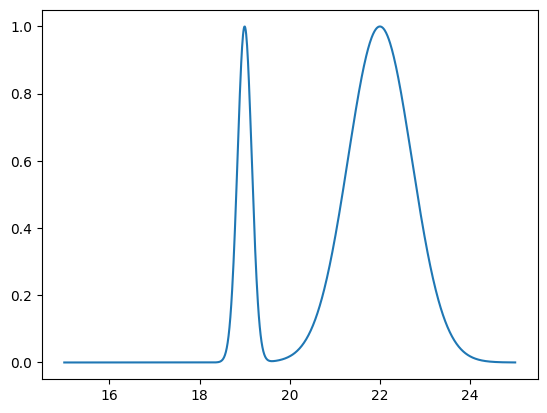
\includegraphics[width = 5cm, height = 5cm]{3-0.png}
		\caption{真解}
		\label{adv0}
	\end{minipage}
	\begin{minipage}{5cm}
		\centering
		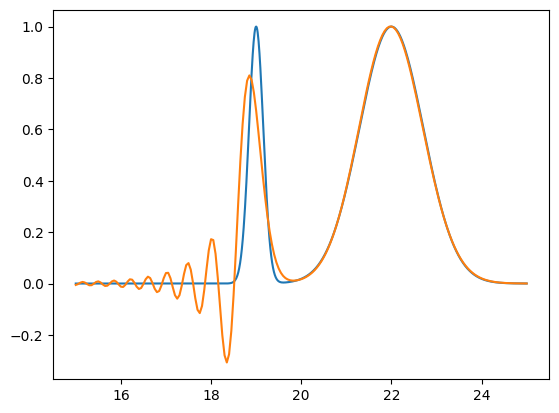
\includegraphics[width = 5cm, height = 5cm]{3-1.png}
		\caption{LeapFrog}
		\label{adv1}
	\end{minipage}
	\begin{minipage}{5cm}
		\centering
		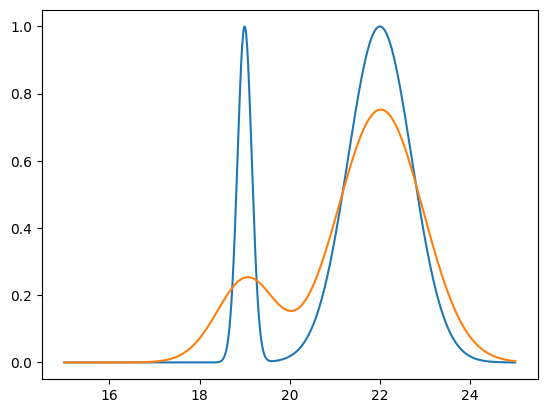
\includegraphics[width = 5cm, height = 5cm]{3-2.png}
		\caption{Lax-Friedrichs}
		\label{adv2}
	\end{minipage}
	\begin{minipage}{5cm}
		\centering
		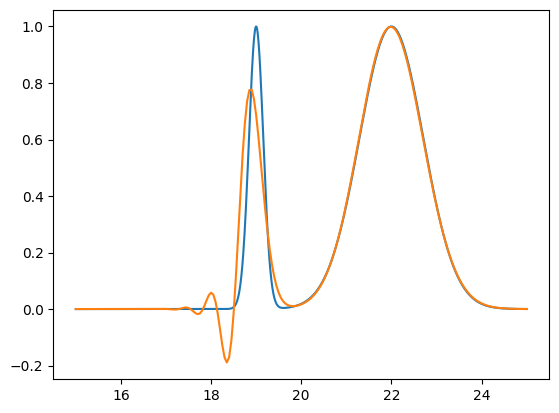
\includegraphics[width = 5cm, height = 5cm]{3-3.png}
		\caption{Lax-Wendroff}
		\label{adv3}
	\end{minipage}
	\begin{minipage}{5cm}
		\centering
		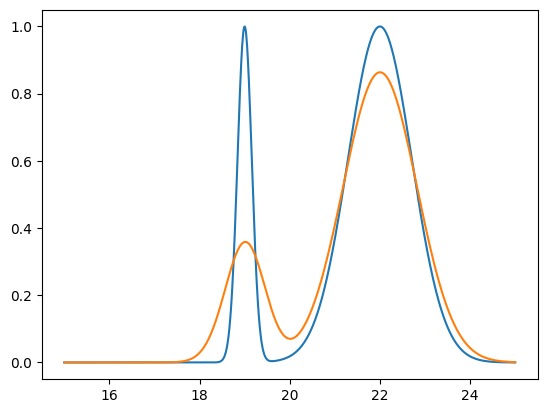
\includegraphics[width = 5cm, height = 5cm]{3-4.png}
		\caption{Upwind}
		\label{adv4}
	\end{minipage}
	\begin{minipage}{5cm}
		\centering
		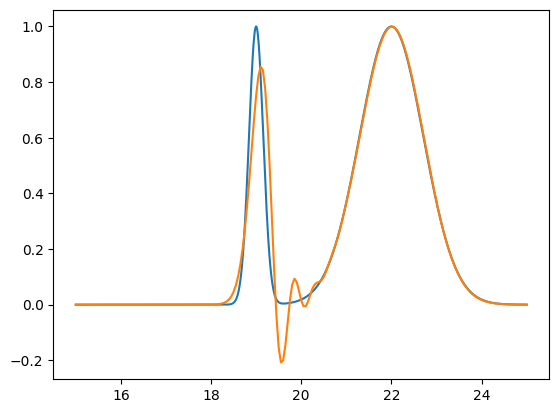
\includegraphics[width = 5cm, height = 5cm]{3-5.png}
		\caption{Beam-Warmer}
		\label{adv5}
	\end{minipage}
\end{figure}

可以发现,尽管$k$和$h$已经取到很小,但各方法的收敛性仍然很差,或出现振荡现象。

虽然各方法都不收敛,但它们的表现有所不同。Upwind方法和Lex-Friedrichs方法的第一个峰没有显现,但图像比较光滑;而另外三种方法的最大模误差稍小,但图像在峰附近反复振荡。

我们知道,事实上,每个方法的依赖域都只有一个点,所以当$k\neq h$即$\mu\neq 1$时,依赖域总会发生较大的偏移。这样造成的误差是无论$k$和$h$取多小都无法有效消除的。因此,对于这些方法,我们也没有必要分析它们的收敛阶。

下面我们取$k=0.05=h$,其他值不变,作图\ref{adv6}到\ref{adv10}:

\begin{figure}[htbp]
	\begin{minipage}{5cm}
		\centering
		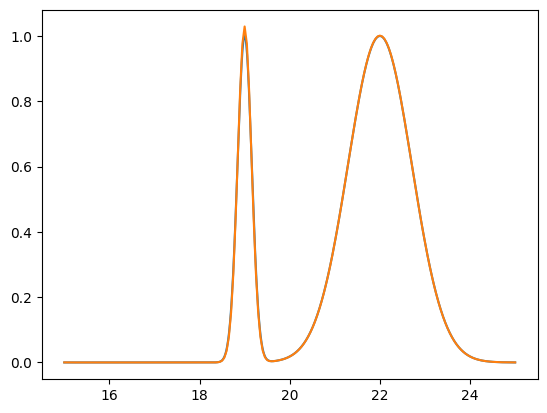
\includegraphics[width = 5cm, height = 5cm]{3-6.png}
		\caption{LeapFrog}
		\label{adv6}
	\end{minipage}
	\begin{minipage}{5cm}
		\centering
		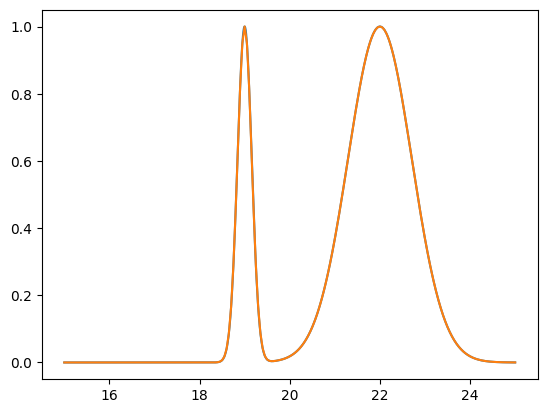
\includegraphics[width = 5cm, height = 5cm]{3-7.png}
		\caption{Lax-Friedrichs}
		\label{adv7}
	\end{minipage}
	\begin{minipage}{5cm}
		\centering
		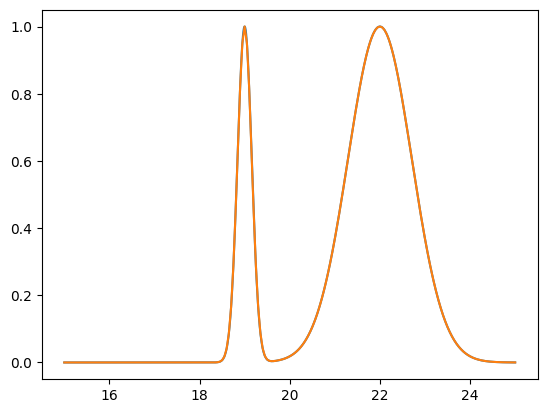
\includegraphics[width = 5cm, height = 5cm]{3-8.png}
		\caption{Lax-Wendroff}
		\label{adv8}
	\end{minipage}
	\begin{minipage}{5cm}
		\centering
		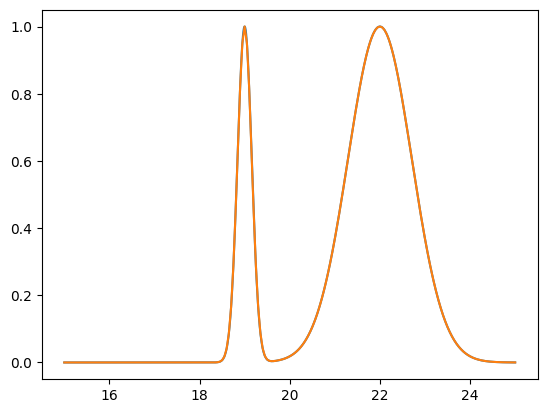
\includegraphics[width = 5cm, height = 5cm]{3-9.png}
		\caption{Upwind}
		\label{adv9}
	\end{minipage}
	\begin{minipage}{5cm}
		\centering
		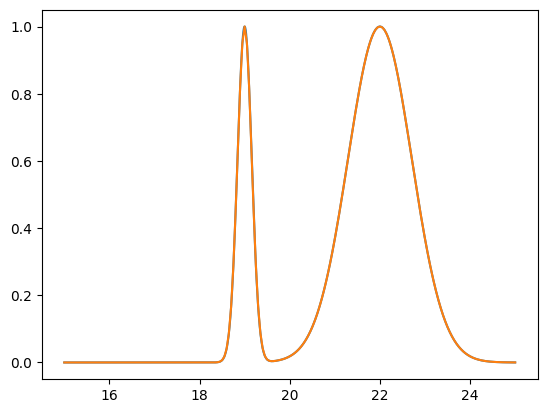
\includegraphics[width = 5cm, height = 5cm]{3-10.png}
		\caption{Beam-Warmer}
		\label{adv10}
	\end{minipage}
\end{figure}

五种方法的数值解图像都几乎和真解重合。事实上,如果我们输出它们误差的精确值可以发现,后四种方法的误差完全相同,均为$2.19\times 10^{-5}$。这是因为当$\mu=1$时,它们本质上就是一种解法(离散格式相同)。LeapFrog方法的误差是$1.84\times 10^-2$。

事实上,此时除LeapFrog外的方法都是二阶收敛的。而LeapFrog方法一阶收敛的原因是第一步的LTE是一阶的。

\end{document}